\section{Benchmarking  for automatized tuning and regression testing}\label{sec:bench}
%
Benchmarking was introduced in \linbox for several reasons. First, It would
give the user a user-friendly way for producing quality graph with no necessary
knowledge of a graphing library like \gnuplot%
%
%
\footnote{\url{http://www.gnuplot.info/}}
%
or provide the \linbox website with automatically updated tables and graphs.
Second, it would be used for regression testing.  Finally, it would be used for
selecting default method, threshold. A lot of libraries do some automatic tuning
at installation (fftw, ATLAS, NTL,\ldots).
%
\par
%
What do we do differently ? Selection between "larger" algorithms, takes more time.
Interpolation.
% XXX BTL\footnote{\url{http://projects.opencascade.org/btl/}}/eigen
%
%
\subsection{Performance evaluation}
%
Our plotting mechanism is based on two structures: {\tt PlotStyle} and {\tt
PlotData}. The  {\tt PlotGraph} structure uses the style and data to manage the
output.  We allow ploting in standard image formats, html and \LaTeX tables,
but also in raw csv or xml. The last raw formats allow for file exchange, data
comparisons and extrapolation.
\danger dave benchmark formats discussion ?
%
\par
%
% \begin{figure}[htbp]
	\centering
	\small
	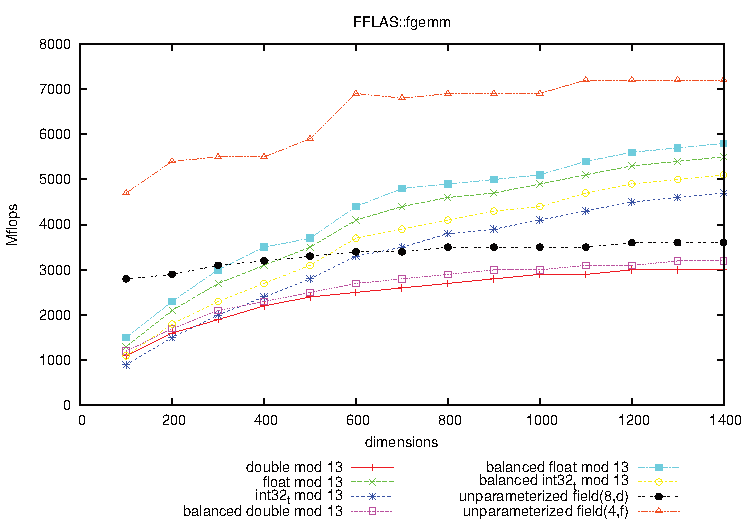
\includegraphics[scale=0.6]{Boyer_Brice/fgemm_square_13_ok}
	\caption{Example of \texttt{benchmark}: \texttt{fgemm}.\label{fig:bench}}
\end{figure}


%
% XXX Time spent on each data is limited (will not start execution if fit (linear least squares) forecasts 'too long'.\\
% XXX Adapts to the environment.
%
\subsection{Automatized regression testing}
%
Saving graphs in raw format can enable automatic regression testing on the
buildbots. For some determined matrices (of different shape and size) over a
few fields, we can accumulate over time the timings for some of our solutions
(rank, det, mul,\ldots). At each new release, when we update the documentation,
we can check any regression on these base cases and automatically update the
regression plots.
\danger We need to implement this framework (not difficult; anybody?).
%JGD: we already have the buildbot, lets focus on this right now
%
\subsection{Automatized tuning and method selection}
%
CPU throttling for ATLAS, \fflasffpack not reliable.
XXX Default are provided, method can be selected via a benchmark (cf wino\_threshold)\\
XXX howto
feature matrix
%JGD: there is already optimiser/winograd.C etc.
